\documentclass[../documentation.tex]{subfiles}

\begin{document}

\newcommand{\const}[1]{\hyperlink{constants}{\texttt{#1}}}
\newcommand{\packet}[1]{\hyperlink{packets}{\texttt{#1}}}

\subsection{Peer Discovery}

\subsubsection{Registration}

When a node starts it generates a random UUID.

When to peers establish a connection, they change a
\packet{RegisterNode} packet. This packet contains information
about their service address and UUID.

\subsubsection{Seeder}

The first step of our peer discovery solution is the \textit{Seeder}.
The Seeder is a server which stores information about node's service addresses.
\\
A node might register himself to a seeder by opening a TCP connection and sending
a \packet{RegisterNode} packet.
Likewise, a node might ask a seeder the service addresses of \textbf{N} nodes by sending a
\packet{RequestNodes} packet.

When the seeder receives a \packet{RegisterNode} it will store its address in the
services pool. The services pool has a fixed capacity of \const{POOL\_CAPACITY}.
Nodes are stored along with their registration timestamp, this means that when the pool
reaches max capacity the oldest node will be uncached. If an already registered node
send a registration packet, the timestamp is updated.
Connection is then closed.

When the seeder receives a \packet{RequestNodes} it will try to randomly draw
as many nodes as requested (max \const{MAX\_REQUEST}) excluding the requester itself.
The \packet{ServeRequestNodes} response packet will be sent back.
Connection is then closed.

It is important to only rely on a seeder when 0 peers are known or when all
the known peers are unreachable.

If a node with an already registered address does register with a new UUID, the old entry is removed.

\subsubsection{Cache}

The nodes will also locally cache some of the peers.
To do so we define the \textit{node} table.

\begin{lstlisting}[style=sql]
    CREATE TABLE IF NOT EXISTS node (
        address VARCHAR(20),
        port INT,
        last_seen_alive DATETIME,
        PRIMARY KEY (address, port)
    );
\end{lstlisting}

When a connection to a peer is established, the node is added to this table.
If the node is already in the database, its \textit{last\_seen\_alive} field is updated.
\\
If the number of nodes in the cache exceeds \const{MAX\_CACHED\_NODES},
the node with the oldest \textit{last\_seen\_alive} field is deleted.

\subsubsection{Algorithm}

A node will actively try to always have \const{MIN\_CONNECTIONS} established connections.
If the number of connections exceeds \const{MAX\_CONNECTIONS}, a random peer is disconnected.

The node will periodically register himself to a random seeder every \const{REGISTER\_INTERVAL} ms.
By doing this dead nodes will stop registering and exit the seeder pool.

\pagebreak

The node will periodically execute the following update every \const{UPDATE\_INTERVAL} ms:

\begin{enumerate}
    \item If peers are less than \const{MIN\_CONNECTIONS}, update from a random peer up to \texttt{MAX\_TRIES\_NEIGHBOUR} times
    \item If peers are less than \const{MIN\_CONNECTIONS}, update from local cache
    \item If peers are \(0\), update from a random seeder up to \const{MAX\_TRIES\_SEEDER} times
\end{enumerate}

\paragraphln{Picking a random seeder}
Seeder addresses are hard-coded in the \const{SEEDERS} array.
Start with a random index, if that seeder is unreachable traverse the array in a circular manner
until one is reachable.

% Circular iterator
\begin{center}
    \begin{tikzcd}
        &&& {\text{rnd}} \\
        {\text{el}_0} & {\text{el}_1} & {\text{el}_2} & {\text{el}_3} & {\text{el}_4}
        \arrow[from=1-4, to=2-4]
        \arrow[from=2-1, to=2-2, bend left=60]
        \arrow[from=2-2, to=2-3, bend left=60]
        \arrow[from=2-4, to=2-5, bend left=60]
        \arrow[from=2-5, to=2-1, bend left=60]
    \end{tikzcd}
\end{center}

\paragraphln{Updating from local cache}
\begin{enumerate}
    \item Read all cached peers from the database
    \item Filter the ones without an estblished connection
    \item While there is still room, try to establish a connection with them
\end{enumerate}

\paragraphln{Updating from seeder}
\begin{enumerate}
    \item Establish a TCP connection with the seeder
    \item Send a \packet{RequestNodes} packet requesting
        \((\text{\const{MIN\_CONNECTIONS}} - \text{\texttt{CONNECTIONS}})\) peers
    \item Filter the ones without an estblished connection
    \item Try to connect to each of them
\end{enumerate}

\paragraphln{Update from a peer}
\begin{enumerate}
    \item Send a \packet{RequestNodes} packet requesting
        \((\text{\const{MIN\_CONNECTIONS}} - \text{\texttt{CONNECTIONS}})\) peers
    \item Filter the ones without an estblished connection
    \item Try to connect to each of them
\end{enumerate}

When a node receives a \packet{RequestNodes}
it will try to randomly draw as many nodes as requested (max
\const{MAX\_REQUEST}) excluding the requester itself.
The \packet{ServeRequestNodes} response packet will be sent back.

\pagebreak

\subsection{Wallet}

\subsubsection{Keypair}

A wallet can be create by generating an \textbf{EdDSA}
(Elliptic Curve Digital Signature Algorithm) keypair
on the \textit{ed25519} curve.

The public key can be retrieved given the private key.

\subsubsection{Address}

The public wallet address is given by the hash of the public key.

\[
    \text{address}=\text{SHA}_{256}(\text{key}_\text{priv})
\]

and the human-readable version

\[
    \text{address}_\text{UTF-8}=\text{base64}(\text{SHA}_{256}(\text{key}_\text{priv}))
\]

\subsection{Mining}

A miner will try to compute the following:

\[
    \theta =
    \text{hash}_\text{last}
    \oplus
    \text{nonce}
    \oplus
    \underset{i}{\oplus}\,
    \text{SHA}_{256}(\text{tx}_i)
\]

Where \(\oplus\) denotes the XOR operator and 
\(\underset{i}{\oplus}\) denotes the XOR over a set,
so \(0 \leq i < \text{length}(\text{tx})\).

A block is mined if a value for \textit{nonce} such that

\[
    \theta < \frac{\const{MAX\_TARGET}}{\text{difficulty}}
\]

is found.

When a peer receives a \packet{SendTransactionPacket} it checks its validity.
If the transaction is valid it gets put into the mempool.
At the arrival of the next valid \packet{PoWSolvedPacket}, the transactions
are drawn from the mempool, inserted into the and inserted into the mining computation.
Finally, at the arrival of the next valid \packet{PoWSolvedPacket}
the transactions will be effectively confirmed.

Since \packet{SendTransactionPacket} packets contain the sender's public key rather than the
address itself, a SQL cache is constructed:

\begin{lstlisting}[style=sql]
	CREATE TABLE IF NOT EXISTS keyCache (
		pub_key BINARY(32),
		address BINARY(32)
	)
\end{lstlisting}

\pagebreak

Here's the SQL table for storing blocks

\begin{lstlisting}[style=sql]
	CREATE TABLE IF NOT EXISTS block (
		id INT PRIMARY KEY,
		difficulty INT,
		tx_hash BINARY(32),
		nonce BINARY(32),
		miner BINARY(32),
		mined DATETIME
	);
\end{lstlisting}

and for storing transactions

\begin{lstlisting}[style=sql]
	CREATE TABLE IF NOT EXISTS tx (
		block_id INT,
		sender_pub BINARY(32),
		recipient BINARY(32),
		amount INT,
		timestamp DATETIME,
		last_tx_hash BINARY(32),
		signature BINARY(64) 
	);
\end{lstlisting}

UTXO can be calculated given every block and transaction,
so here's a table to cache this value.

\begin{lstlisting}[style=sql]
	CREATE TABLE IF NOT EXISTS wallet (
		address BINARY(32),
		amount INT
	)
\end{lstlisting}

\subsection{Nodes}

There are three types of nodes:

\begin{itemize}
    \item \textbf{Full Node} Full functional node
    \item \textbf{Mining Node} Node that produces Proof-of-Works
    \item \textbf{API Node} Node with HTTP POST routes
\end{itemize}

Both miner node and API node extend the full node, so they are both also functional full nodes.

\begin{center}
    \begin{tikzpicture}[font=\ttfamily,
        mymatrix/.style={matrix of nodes, nodes=typetag, row sep=1em},
        mycontainer/.style={draw=gray, inner sep=1ex},
        typetag/.style={draw=gray, inner sep=1ex, anchor=west},
        title/.style={draw=none, color=gray, inner sep=0pt}
        ]
        \matrix[mymatrix] (mx1) {
            |[title]|API Node \phantom{g} \\ % \phantom{g} to add an invisible g
                                             % otherwise m2 is taller
            Full Node \\
        };
        \matrix[mymatrix, right=of mx1.north east, matrix anchor=north west] (mx2) {
            |[title]|Mining Node \\
            Full Node \\
        };
        \matrix[mymatrix, right=of mx2.north east, matrix anchor=north west] (mx3) {
            |[title]|Full Node \\
        };
    
        \node[mycontainer, fit=(mx1)] {};
        \node[mycontainer, fit=(mx2)] {};
        \node[mycontainer, fit=(mx3)] {};
    \end{tikzpicture}
\end{center}

Here is a table of what each node type knows and can do.

\bgroup{}
\def\arraystretch{1.25}
\begin{center}
    \begin{tabular}{ |c|c|c|c| }
        \hline
        &
        \textbf{\makecell[c]{Makes new \\ blocks}} &
        \textbf{\makecell[c]{Deploys \\ transactions}} &
        \textbf{\makecell[c]{knows all \\ transactions}} \\
        \hline
        \makecell[l]{Full Node} & - & - & + \\
        \hline
        \makecell[l]{API Node} & - & + & + \\
        \hline
        \makecell[l]{Mining Node} & + & - & + \\
        \hline
    \end{tabular}
\end{center}
\egroup{}

\pagebreak

\subsection{Difficulty}

Difficulty is adjusted every \const{DIFFICULTY\_ADJUSTMENT\_RATE} blocks.
The difficulty is adjusted such that the time to mine a block is 
approximately \const{BLOCK\_RATE} ms.
Every adjustament is based on the last \const{DIFFICULTY\_ADJUSTMENT\_DEPTH} blocks.

\[
    \text{difficulty}_\text{new} =
    \text{difficulty}_\text{old} \cdot
    \frac{\const{BLOCK\_RATE}\cdot\const{DIFFICULTY\_ADJUSTMENT\_DEPTH}}
    {\Delta(\const{DIFFICULTY\_ADJUSTMENT\_DEPTH})} 
\]

where \(\Delta (x)\) is the time to mine the last \(x\) blocks.

\subsection{Blockchain download}

When a node joins the network, either for the first time
or after some time of being offline, it needs to download
all the transactions and new blocks.

Furthermore, in the event of a branch of the blockchain, the branch
that will first reach a higher length than the other must be adopted
by every node hosting the other branch.

To accomplish so, each peer periodically asks his neighbours for their blockchain length.
If their length is greater than his (and there is consensus) it will try to establish a common block
and download the peer's blockchain starting from that block.

\begin{center}
    \begin{tikzpicture}
        \path 
        (0,0) node (b1) {\(1\)}
        (1,0) node (b2) {\(2\)}
        (2,0) node (b3) {\(3\)}
        (3,0) node (b4) {\(4\)}
        (0,2) node (a1) {\(1\)}
        (1,2) node (a2) {\(2\)}
        (2,2) node (a3) {\(3\)}
        (3,2) node (a4) {\(4\)}
        (4,2) node (a5) {\(5\)}
        (5,2) node (a6) {\(6\)};
        \node[draw,fit=(b1) (b1)] (c1) {};
        \node[draw,fit=(b2) (b2)] (c2) {};
        \node[draw,fit=(b3) (b3)] (c3) {};
        \node[draw,fit=(b4) (b4)] (c4) {};
        \node[draw,fit=(a1) (a1)] (c5) {};
        \node[draw,fit=(a2) (a2)] (c6) {};
        \node[draw,fit=(a3) (a3)] (c7) {};
        \node[draw,fit=(a4) (a4)] (c8) {};
        \node[draw,fit=(a5) (a5)] (c9) {};
        \node[draw,fit=(a6) (a6)] (c10) {};
        \node[draw] at (4,1) {Last common block};
        \draw[->] (c1)--(c2);
        \draw[->] (c2)--(c3);
        \draw[->] (c3)--(c4);
        \draw[->] (c5)--(c6);
        \draw[->] (c6)--(c7);
        \draw[->] (c7)--(c8);
        \draw[->] (c8)--(c9);
        \draw[->] (c9)--(c10);
        \draw[thick, darkgreen, <->] (c3)--(c7);
    \end{tikzpicture}    
\end{center}

Once the common block has been found the other peer will start sending
\packet{ServeOldTransactionPacket} and \packet{ServeOldPoWPacket} packets in the correct order.
The peer will also send transactions currently in the mempool. Finally, the peer sends a
\packet{DownloadDonePacket}.

A peer will not send a download request if the lengths are the same, except
at startup (so that the mempool is updated and kept up to date).

\subsubsection{Finding common node}

Start by sending a \packet{RequestIsHashExistsPacket} containing the hash of the last block
available. If the response block ID is positive (not \(-1\), this is the last common block.
Otherwise, try the same thing with the block before. If the iteration exceeds a depth of \(5\),
set the common ID to be 0.

\pagebreak

\subsubsection{Hashing}

Here are the effective hashes for a block and for a transaction

\paragraph{Block}

\begin{align*}
    \text{block}_\text{hash} &=
    \text{SHA}_{256}(\text{id}) \\
    &\oplus \text{SHA}_{256}(\text{difficulty}) \\
    &\oplus \text{SHA}_{256}(\text{tx}_\text{hash}) \\
    &\oplus \text{SHA}_{256}(\text{nonce}) \\
    &\oplus \text{SHA}_{256}(\text{miner}) \\
    &\oplus \text{SHA}_{256}(\text{last}_\text{hash}) \\
    &\oplus \text{SHA}_{256}(\text{timestamp})
\end{align*}

\paragraph{Transaction}

\begin{align*}
    \text{block}_\text{hash} &=
    \text{SHA}_{256}(\text{sender}_\text{public}) \\
    &\oplus \text{SHA}_{256}(\text{recipient}) \\
    &\oplus \text{SHA}_{256}(\text{amount}) \\
    &\oplus \text{SHA}_{256}(\text{last}_\text{hash}) \\
    &\oplus \text{SHA}_{256}(\text{signature})
\end{align*}

\pagebreak

\hypertarget{constants}{}
\subsection{Constants}

Here is a list of hard-coded values and constants.

\paragraphln{Database}
Constants related to the database node caching

\bgroup{}
\def\arraystretch{1.25}
\begin{tabular}{|l|l|}
    \hline
    \textbf{Name} & \textbf{Default}
    \\ \hline
    MAX\_CACHED\_NODES & 50
    \\ \hline
\end{tabular}
\egroup{}

\paragraphln{Seeder}
Constants related to the seeder

\bgroup{}
\def\arraystretch{1.25}
\begin{tabular}{|l|l|}
    \hline
    \textbf{Name} & \textbf{Default}
    \\ \hline
    POOL\_CAPACITY & 100
    \\ \hline
    MAX\_REQUEST & 10
    \\ \hline
\end{tabular}
\egroup{}

\paragraphln{Blockchain}
Constants related to the blockchain system:

\bgroup{}
\def\arraystretch{1.25}
\begin{tabular}{|l|l|}
    \hline
    \textbf{Name} & \textbf{Default}
    \\ \hline
    BLOCK\_REWARD & 1000
    \\ \hline
    BLOCK\_RATE & 20000
    \\ \hline
    DIFFICULTY\_ADJUSTMENT\_RATE & 5
    \\ \hline
    DIFFICULTY\_ADJUSTMENT\_DEPTH & 6
    \\ \hline
    INITIAL\_DIFFICULTY & 1
    \\ \hline
    MAX\_TARGET & \(15 \cdot 2^{248}\)
    \\ \hline
\end{tabular}
\egroup{}

\paragraphln{Node}
Constants related to the peer connections:

\bgroup{}
\def\arraystretch{1.25}
\begin{tabular}{|l|l|}
    \hline
    \textbf{Name} & \textbf{Default}
    \\ \hline
    MAX\_CONNECTIONS & 150
    \\ \hline
    MIN\_CONNECTIONS & 100
    \\ \hline
    REGISTER\_INTERVAL & 180000
    \\ \hline
    UPDATE\_INTERVAL & 180000
    \\ \hline
    MAX\_TRIES\_SEEDER & 5
    \\ \hline
    MAX\_TRIES\_NEIGHBOUR & 5
    \\ \hline
    DEFAULT\_PORT & 5555
    \\ \hline
    SEEDERS & \makecell[t] {
        127.0.0.1:4670 \\
        127.0.0.1:4671 \\
        127.0.0.1:4672
    }
    \\ \hline
\end{tabular}
\egroup{}

\pagebreak

\paragraphln{Packets IDs}

\bgroup{}
\def\arraystretch{1.25}
\begin{tabular}{|l|c|}
    \hline
    \textbf{Name} & \textbf{Default}
    \\ \hline
    REQUEST\_NODES & 0x0
    \\ \hline
    SERVE\_NODES & 0x1
    \\ \hline
    REGISTER\_NODE & 0x2
    \\ \hline
    SEND\_TRANSACTION & 0x3
    \\ \hline
    REQUEST\_BLOCKCHAIN\_LENGTH & 0x4
    \\ \hline
    SERVE\_BLOCKCHAIN\_LENGTH & 0x5
    \\ \hline
    REQUEST\_IF\_HASH\_EXISTS & 0x6
    \\ \hline
    SERVE\_IF\_HASH\_EXISTS & 0x7
    \\ \hline
    POW\_SOLVED & 0x8
    \\ \hline
    REQUEST\_DOWNLOAD & 0x9
    \\ \hline
    SERVE\_OLD\_TX & 0xA
    \\ \hline
    SERVE\_OLD\_POW & 0xB
    \\ \hline
    DOWNLOAD\_DONE & 0xC
    \\ \hline

\end{tabular}
\egroup{}

\hypertarget{packets}{}
\subsection{Packets}

Packets are sent over a TCP socket stream.
Each packet is preceded by the length of the packet,
encoded as a Little-Endian 32-bit integer.


\newcommand{\tline}{
    \\ \hline
}

\newcommand{\packettabular}[1]{
    \bgroup{}
    \def\arraystretch{1.25}
    \begin{center}
        \begin{tabular}{|l|l|l|}
            \hline
            \textbf{Name} & \textbf{Type} & \textbf{Descritpion}
            \tline
            ID & u8 & Packet Identifier
            \tline

            \if\relax\detokenize{#1}\relax
                % if arg is empty
            \else
                #1
                \tline
            \fi
        \end{tabular}
    \end{center}
    \egroup{}
}

\newcommand{\packettabularnoid}[1]{
    \bgroup{}
    \def\arraystretch{1.25}
    \begin{center}
        \begin{tabular}{|l|l|l|}
            \hline
            \textbf{Name} & \textbf{Type} & \textbf{Descritpion}
            \tline

            \if\relax\detokenize{#1}\relax
                % if arg is empty
            \else
                #1
                \tline
            \fi
        \end{tabular}
    \end{center}
    \egroup{}
}

\subsubsection{DownloadDonePacket}

This package indicates that the requested download has ended.

\packettabular{}

\subsubsection{PoWSolvedPacket}

A miner will broadcast this packet when he mines a block.

\packettabular{
    nonce & blob & The mined nonce
    \tline
    miner & blob & Address of the miner
    \tline
    timestamp & u64 & Timestamp
}

\subsubsection{RegisterNodePacket}

Used to register the node service to another peer or a seedeer.

\packettabular{
    port & u16 & The port of the service
    \tline
    uuid & UUID & The UUID of the node
}

\subsubsection{RequestBlockchainLengthPacket}

Used to request the length of the blockchain to a peer.

\packettabular{}

\subsubsection{RequestDownloadPacket}

Used to request download of new blocks, transactions and mempool
from a peer.

\packettabular{
    port & i32 & Starting block ID
}

\subsubsection{RequestIfHashExistsPacket}

Used to ask a peer wheter a certian hash exists in his blockchain.

\packettabular{
    hash & blob & Hash
}

\subsubsection{RequestNodesPacket}

Used to request peers addresses to a peer or a seeder.

\packettabular{
    amount & u32 & Requested amount
    \tline
    exclude & UUID & UUID to exclude
}

\subsubsection{SendTransactionPacket}

This packet is broadcasted when a node wants to deploy a transaction.

\packettabular{
    timestamp & u64 & The timestamp
    \tline
    recipient & blob & Recipient address
    \tline
    sender\_pub & blob & Sender public key
    \tline
    amount & u64 & The amount of the transaction
    \tline
    last\_tx\_hash & blob & The hash of the last transaction
    \tline
    signature & blob & The signature
}

\subsubsection{ServeBlockchainLengthPacket}

Used to serve the blockchain length to a peer.

\packettabular{
    length & i32 & Blockchain length
}

\subsubsection{ServeIfHashExistsPacket}

Used to serve the result of a block hash search.
If the hash is found this packet will contain the block ID.
The block ID is \(-1\) otherwise.

\packettabular{
    id & i32 & Block ID
}

\subsubsection{ServeNodesPacket}

This packet is used to serve the requested nodes addresses.

\packettabular{
    amount & i32 & Amount of nodes
    \tline
    nodes & node\ldots & Node addresses
}

\subsubsection{ServeOldPoWPacket}

This packet is used to serve an old Proof-of-Work packet.

\packettabular{
    nonce & blob & The mined nonce
    \tline
    miner & blob & Address of the miner
    \tline
    timestamp & u64 & Timestamp
}

\subsubsection{ServeOldTransactionPacket}

This packet is used to serve an old trasaction packet.

\packettabular{
    timestamp & u64 & The timestamp
    \tline
    recipient & blob & Recipient address
    \tline
    sender\_pub & blob & Sender public key
    \tline
    amount & u64 & The amount of the transaction
    \tline
    last\_tx\_hash & blob & The hash of the last transaction
    \tline
    signature & blob & The signature
}

\subsection{Encodings}

Here's a certain types are encoded. \\
Types from u16 to i64 are encoded in Little-Endian format.

\subsubsection{Blob}

Encoding of binary data.

\packettabularnoid{
    length & i32 & Data size
    \tline
    data & u32\ldots & Blob data
}

\subsubsection{UUID}

Encoding of a UUID value.

\packettabularnoid{
    left & u64 & Left-most bits
    \tline
    right & u64. & Right-most bits
}

\subsubsection{Node}

Encoding of a node service address.

\packettabularnoid{
    address & string & Address string
    \tline
    port & u16. & Port
}

\subsubsection{String}

Encoding of a string value.

\packettabularnoid{
    length & u8 & String length
    \tline
    data & u8\ldots & String UTF-8 chars
}

\subsection{Interactions}

Interactions between nodes when a packet is sent.

\bgroup{}
\def\arraystretch{1.25}
\begin{center}
    \begin{tabular}{|l|l|}
        \hline
        \textbf{Packet sent} & \textbf{Response}
        \\ \hline
        \packet{PoWSolvedPacket} & 
        \\ \hline
        \packet{RegisterNodePacket} &
        \\ \hline
        \packet{RequestBlockchainLengthPacket} & \packet{ServeBlockchainLengthPacket}
        \\ \hline
        \packet{RequestDownloadPacket} & (\packet{ServeOldPowPacket} | \packet{ServeOldTransactionPacket}) + \packet{DownloadDonePacket}
        \\ \hline
        \packet{RequestIfHashExistsPacket} & \packet{ServeIfHashExistsPacket}
        \\ \hline
        \packet{RequestNodesPacket} & \packet{ServeNodesPacket}
        \\ \hline
        \packet{SendTransactionPacket} &
        \\ \hline
    \end{tabular}
\end{center}
\egroup{}

\pagebreak

\subsection{API}

The API node has some HTTP POST routes to interact with the blockchain.

\paragraphln{Blockchain Height}

Returns the height of the blockchain.
\\
Route: \texttt{/getBlockchainHeight}
\\
Example:
\begin{lstlisting}[language=json]
    {
        "status": "Ok",
        "height": 3
    }
\end{lstlisting}

\subsubsection{Get Block}

Returns the block data given its ID.
\\
Route: \texttt{/getBlock/<id>}
\\
Example:
\begin{lstlisting}[language=json]
    {
        "status": "Ok",
        "nonce": "iKU71ffO++lmUKvJNwxyM3x/gOgjoiqlyvRxIcTKmCk=",
        "difficulty": 368273
        "miner": "ZZ1PjoBwOZQGP0AYPmwxHsa5Z9YhRDaDbE1XIKyCUsA=",
        "timestamp": 1651363707165,
        "last_hash": "AvM6wrrEZL29GGMigfkCzflUN54yrX/jQZXImkFpcAI=",
        "hash": "6TrC8QKdegOvnonbaFQJhG6DZddkMaXwoOdst9tC+8w=",
        "nTx": 0
    }
\end{lstlisting}

\subsubsection{Get UTXO}

Returns the UTXO of a wallet given its address.
\\
Route: \texttt{/getUTXO/<address>}
\\
Example:
\begin{lstlisting}[language=json]
    {
        "status": "Ok",
        "utxo": 1500
    }
\end{lstlisting}

\pagebreak

\subsubsection{Get Transaction}

Returns the transaction data given its hash.
\\
Route: \texttt{/getTx/<hash>}
\\
Example:
\begin{lstlisting}[language=json]
    {
        "status": "Ok",
        "blockId": 3,
        "sender": "ZZ1PjoBwOZQGP0AYPmwxHsa5Z9YhRDaDbE1XIKyCUsA=",
        "recipient": "SQAf8paS6Rr5nnd5dC8Bx5h6YKzdAd0Y0g9UMrTa378=",
        "amount": 500,
        "timestamp": 1651363700693,
        "lastTxHash": "AAAAAAAAAAAAAAAAAAAAAAAAAAAAAAAAAAAAAAAAAAA=",
        "signature": "Z0n8TA1zenp+U0ONzSAJLot3JZ5GUedPvViW8vCN8Q6h
                      vmqB81lHsTFg4g7Gb9DFMcnB8KK6TcknAbIAfZTrBg==",
        "hash": "MmVCpq21pR/ZLYZwjaMF0AdyRVImq2YZ4MqO9mstnzw="
    }
\end{lstlisting}

\subsubsection{Deploy Transaction}

Broadcasts a transaction packet to the network.
\\
Route: \texttt{/deploy}
\\
The packet data is in the HTTP body.

\subsubsection{Get Transactions}

Returns the list of all transactions received or spent by a given address.
\\
Route: \texttt{/getTxs/<address>}
\\
Example:
\begin{lstlisting}[language=json]
    {
        "status": "Ok",
        "txs":[
            {
                "blockId": 3,
                "sender": "ZZ1PjoBwOZQGP0AYPmwxHsa5Z9YhRDaDbE1XIKyCUsA=",
                "recipient": "SQAf8paS6Rr5nnd5dC8Bx5h6YKzdAd0Y0g9UMrTa378=",
                "amount": 500,
                "timestamp": 1651363700693,
                "lastTxHash": "AAAAAAAAAAAAAAAAAAAAAAAAAAAAAAAAAAAAAAAAAAA=",
                "signature": "Z0n8TA1zenp+U0ONzSAJLot3JZ5GUedPvViW8vCN8Q6hv
                              mqB81lHsTFg4g7Gb9DFMcnB8KK6TcknAbIAfZTrBg==",
                "hash": "MmVCpq21pR/ZLYZwjaMF0AdyRVImq2YZ4MqO9mstnzw="
            }
        ]
    }
\end{lstlisting}

\pagebreak

\subsubsection{Get last Transaction}

Returns the last spent transaction from a given wallet.
\\
Route: \texttt{/getLastTx/<address>}
\\
Example:
\begin{lstlisting}[language=json]
    {
        "status": "Ok",
        "blockId": 4,
        "sender": "ZZ1PjoBwOZQGP0AYPmwxHsa5Z9YhRDaDbE1XIKyCUsA=",
        "recipient": "SQAf8paS6Rr5nnd5dC8Bx5h6YKzdAd0Y0g9UMrTa378=",
        "amount": 500,
        "timestamp": 1651363715045,
        "lastTxHash": "Bd+Wlarl0kNjxX8ZpvFKaNA0MNjwY2RSUzKrk/iksxQ=",
        "signature": "VEgzDvWkS+/T4Tt2RBdq/4TZv5Wv6L7dxf7Xb3WqcxV0
                      svYdL/fxde3N34x04KoilvqifQ0MfqP4Nt+nntYeBw==",
        "hash": "reAXKECxKhTfpEE/60nrfD+UgYURGka5Wl97XjlrSUg="
    }
\end{lstlisting}

\subsubsection{Error responses}

When the ID/Address/Hash is not found

\begin{lstlisting}[language=json]
    {
        "status": "Not Found"
    }
\end{lstlisting}

When the address is invalid

\begin{lstlisting}[language=json]
    {
        "status": "Invalid Address"
    }
\end{lstlisting}

When the hash is invalid

\begin{lstlisting}[language=json]
    {
        "status": "Invalid Hash"
    }
\end{lstlisting}

When the ID is invalid

\begin{lstlisting}[language=json]
    {
        "status": "Invalid ID"
    }
\end{lstlisting}

\subsubsection{Other}

The slash character \texttt{/} must be replaced with \texttt{\%2F} in the URL.

\pagebreak

\subsection{Website}

The website interact with an API node to display informations about the blockchain
and deploy transactions.

The address of the API node is in \texttt{website-frontend/js/post.js}

\subsubsection{Dependency table}

The website relies on various libraries, some of which are not stored locally.
This means that the user will query third-party servers, thus the website will not work
locally if you do not have a free internet connection.

\medskip

\bgroup{}
\def\arraystretch{1.5}
\begin{center}
    \begin{tabular}{ |p{3cm}|p{4cm}|p{2cm}|p{2cm}| }
        \hline
        \multicolumn{4}{|c|}{\textbf{Dependency table}} \\
        \hline
        \textbf{Name} & \textbf{Description} & \textbf{Stored} & \textbf{Version} \\
        \hline
        Bootstrap (CSS) & Styling framework & Locally & 5.1.3 \\
        \hline
        Bootstrap (JS) & Styling framework & Remotely & 4.6.1 \\
        \hline
        Dropzone.js & File drop & Remotely & 1.0 \\
        \hline
    \end{tabular}
\end{center}
\egroup{}

\pagebreak

\subsubsection{Design}

\paragraphln{Homepage}

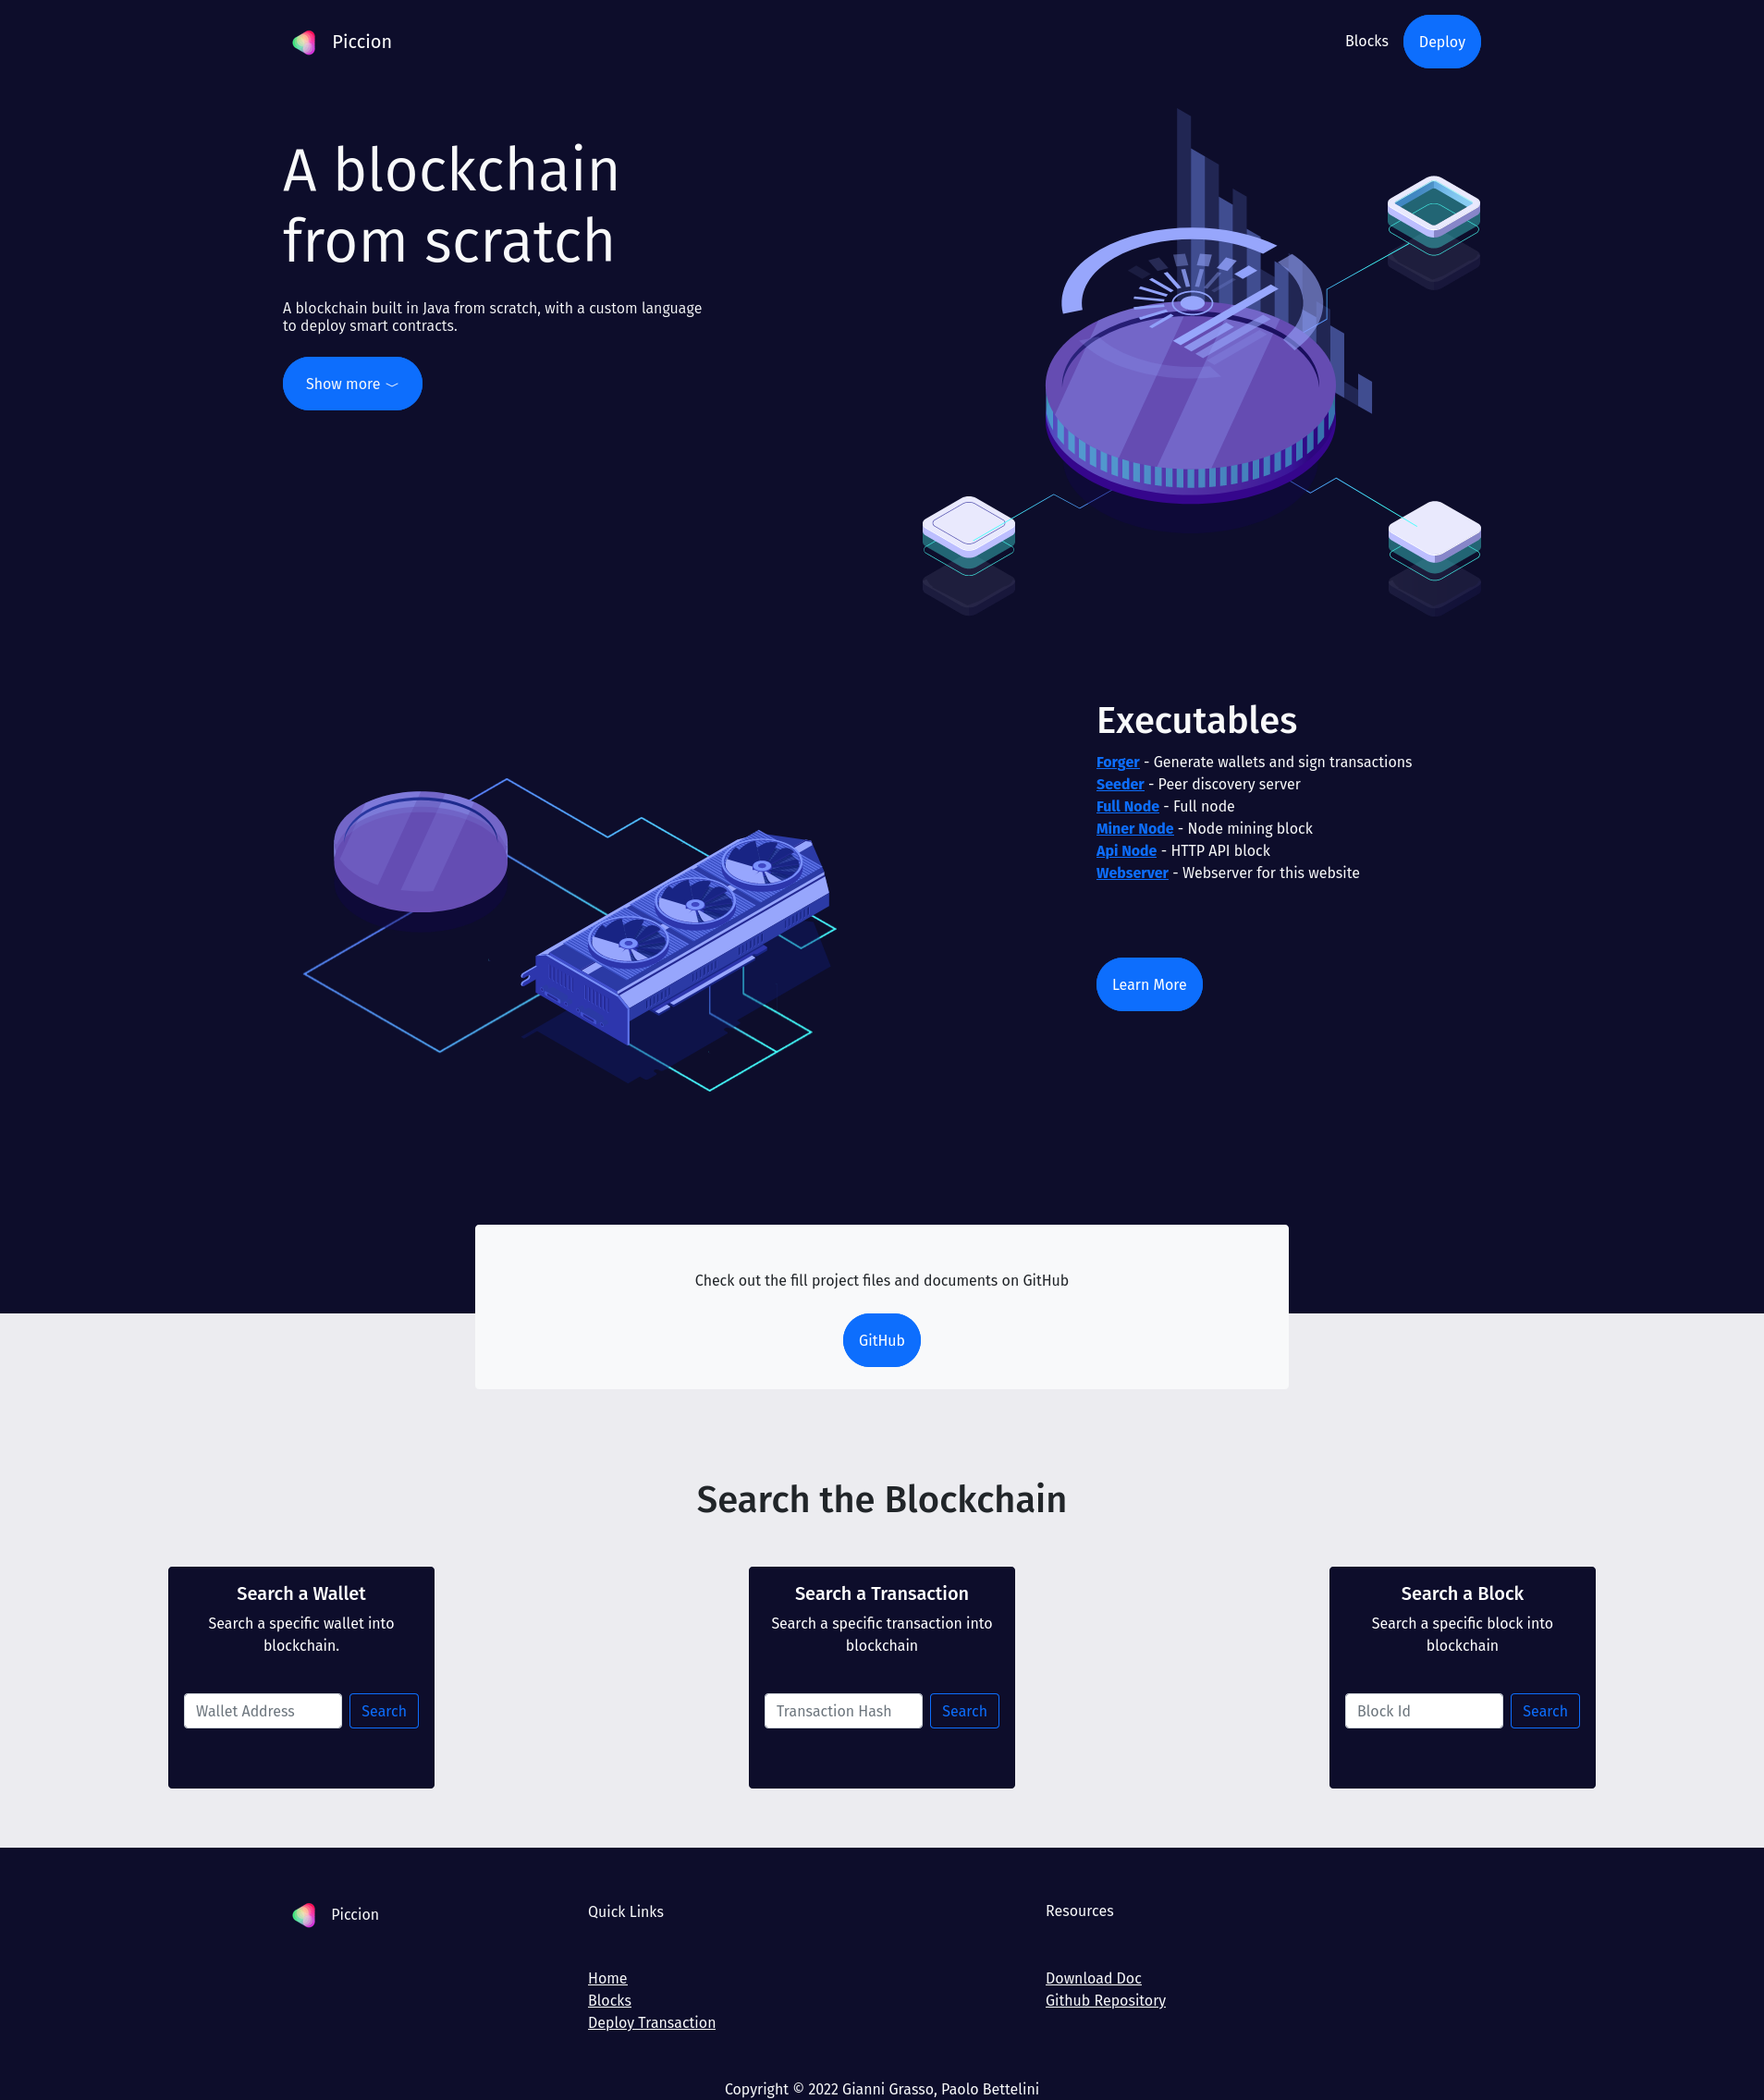
\includegraphics[width=\textwidth]{images/website1}

\paragraphln{Blocks}

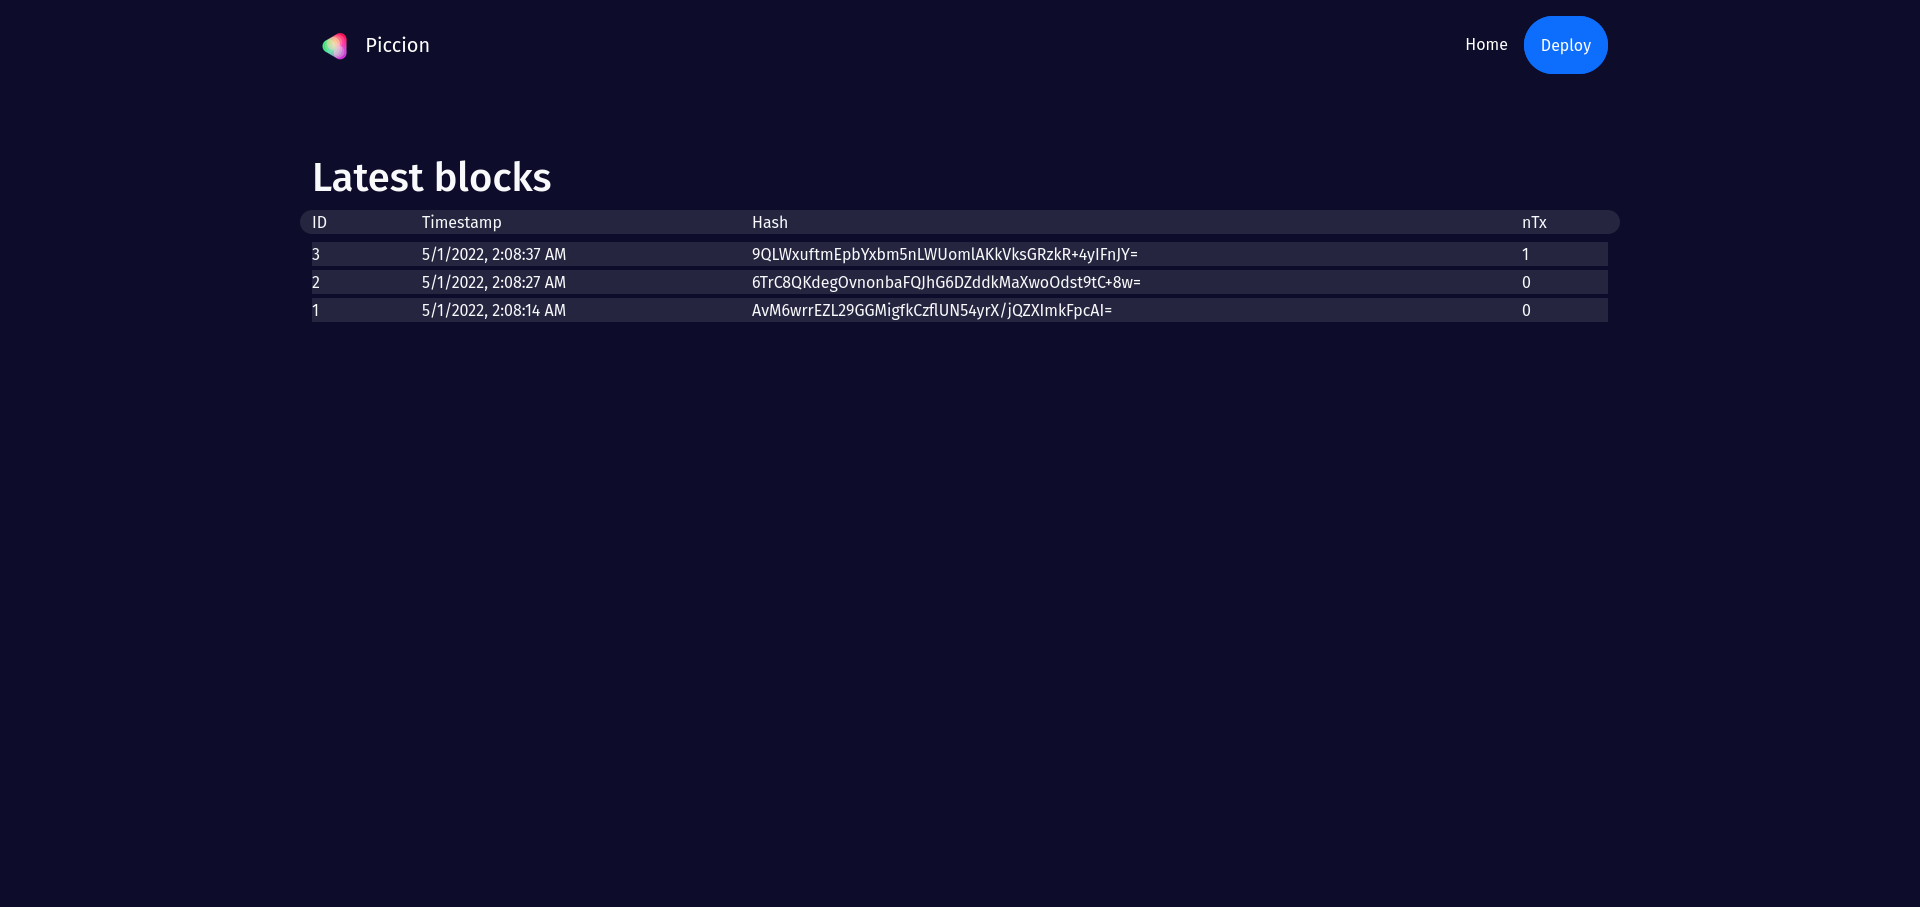
\includegraphics[width=\textwidth]{images/website2}

\paragraphln{Block}

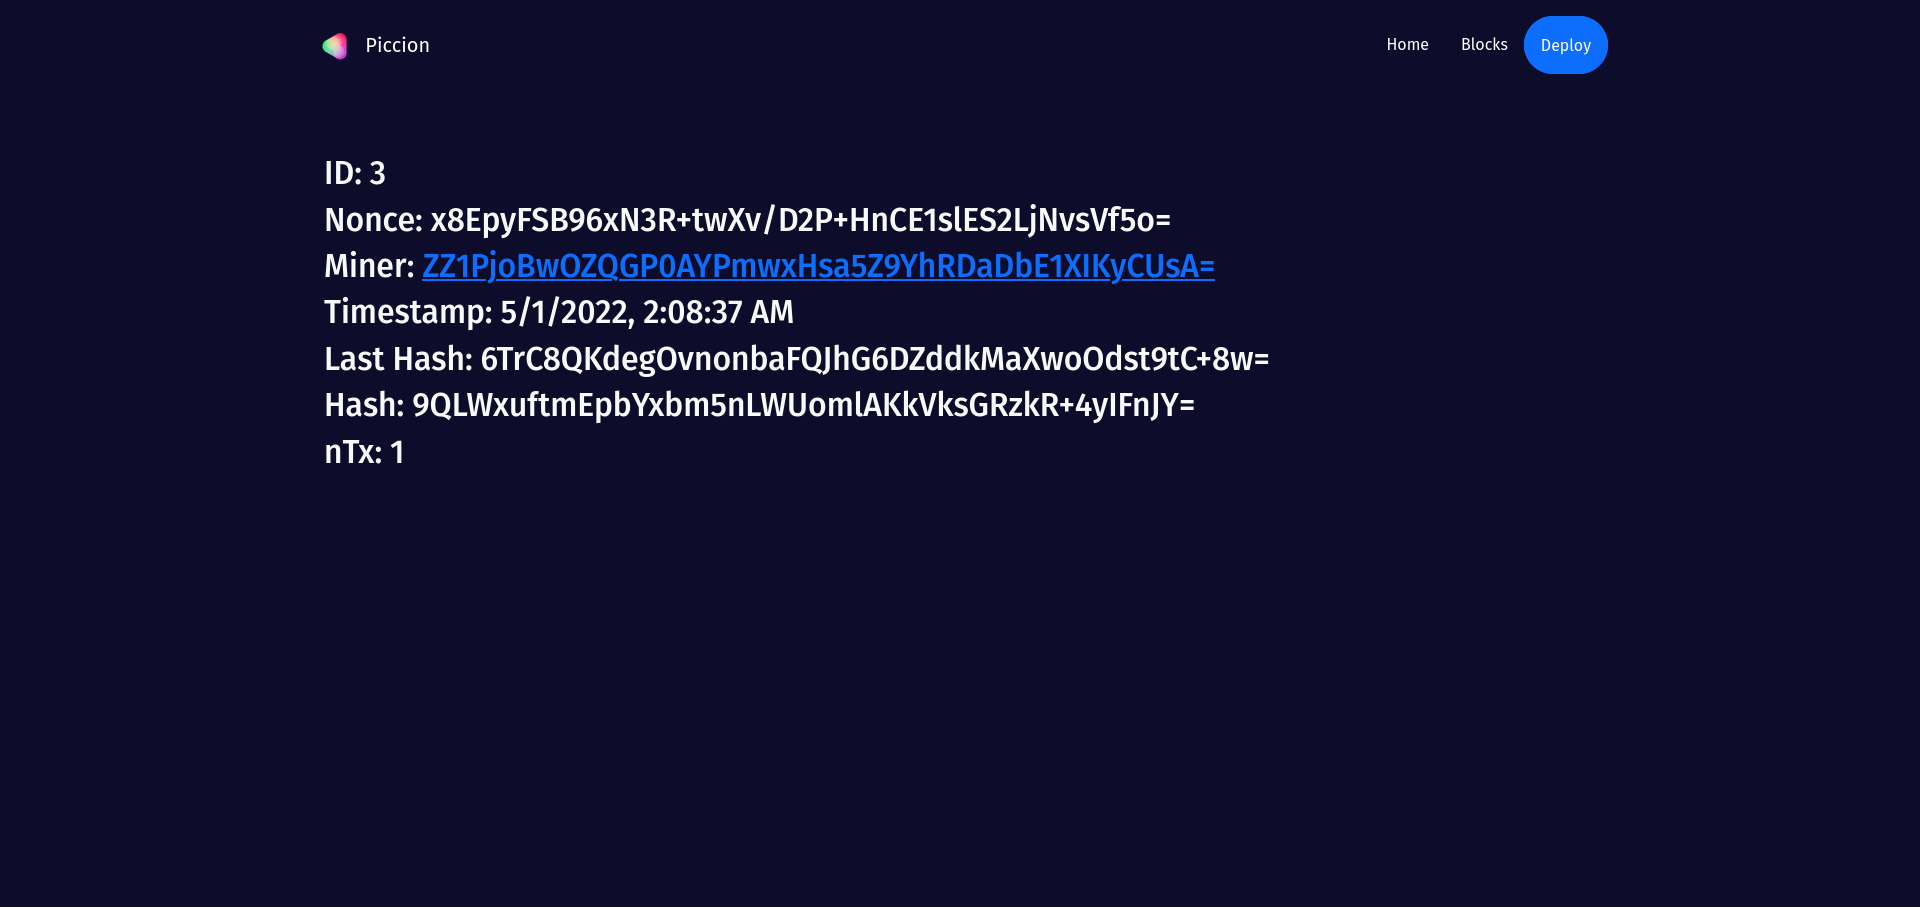
\includegraphics[width=\textwidth]{images/website3}

\pagebreak

\paragraphln{Wallet}

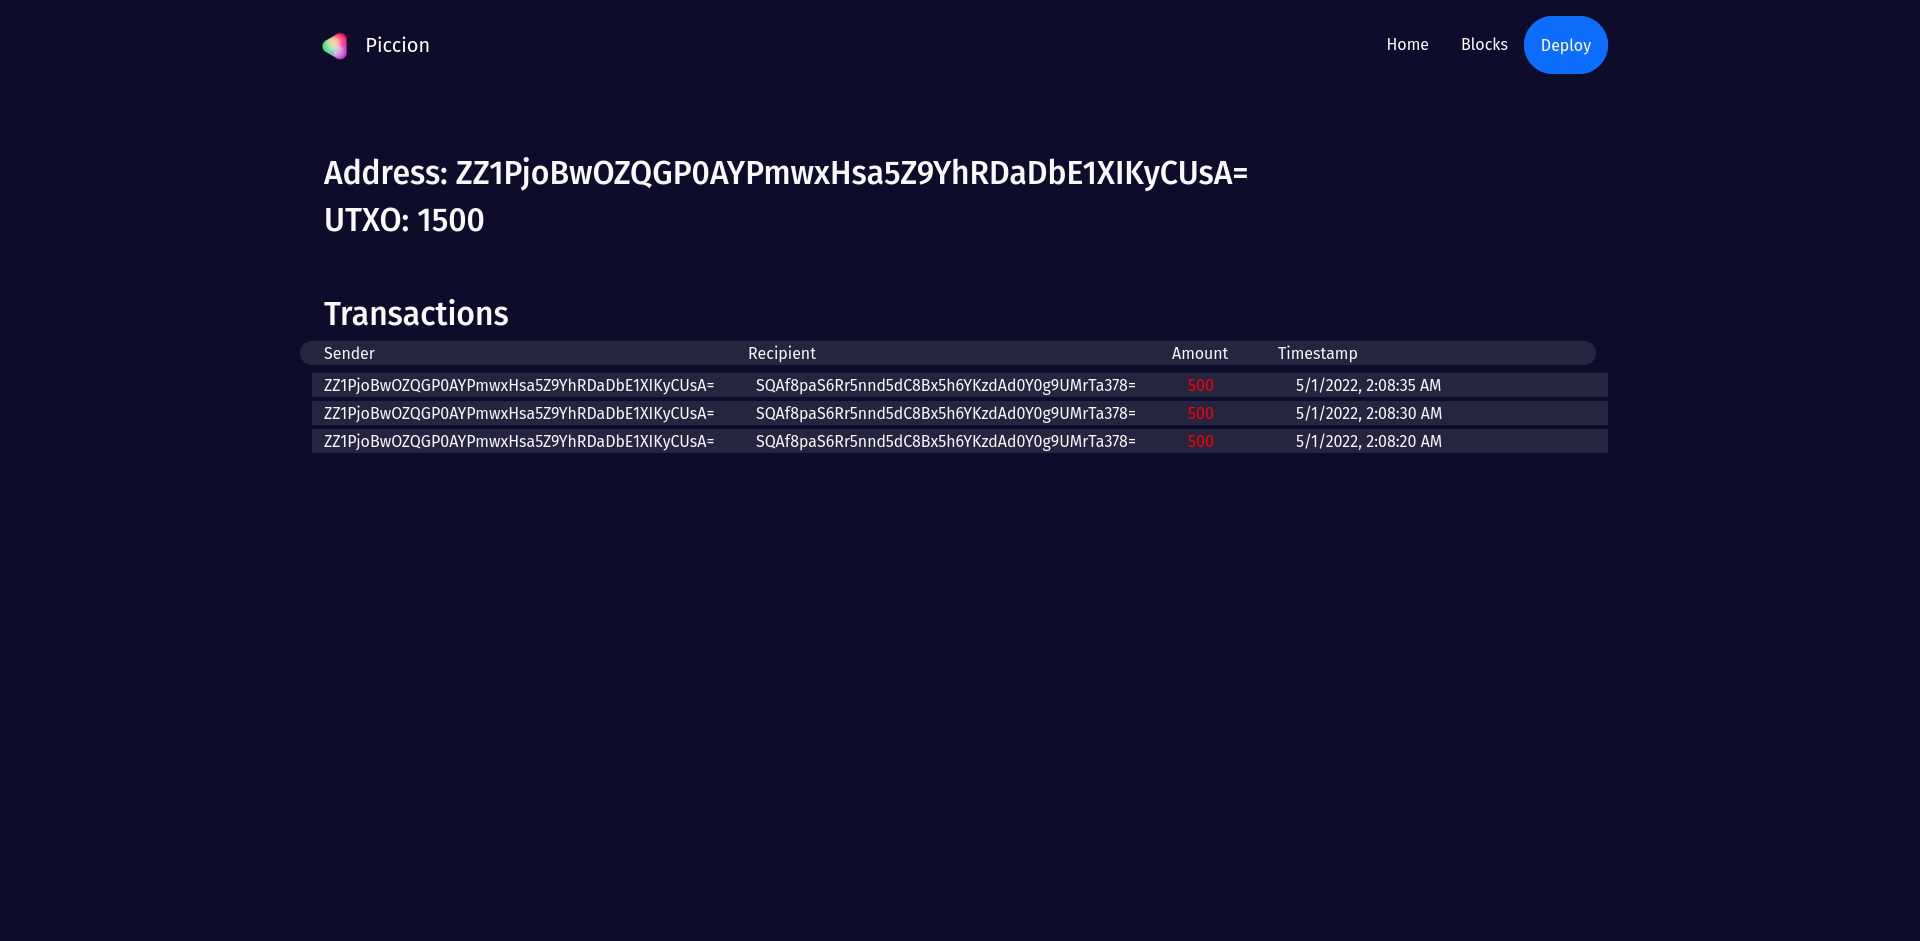
\includegraphics[width=\textwidth]{images/website4}

\paragraphln{Deploy page}

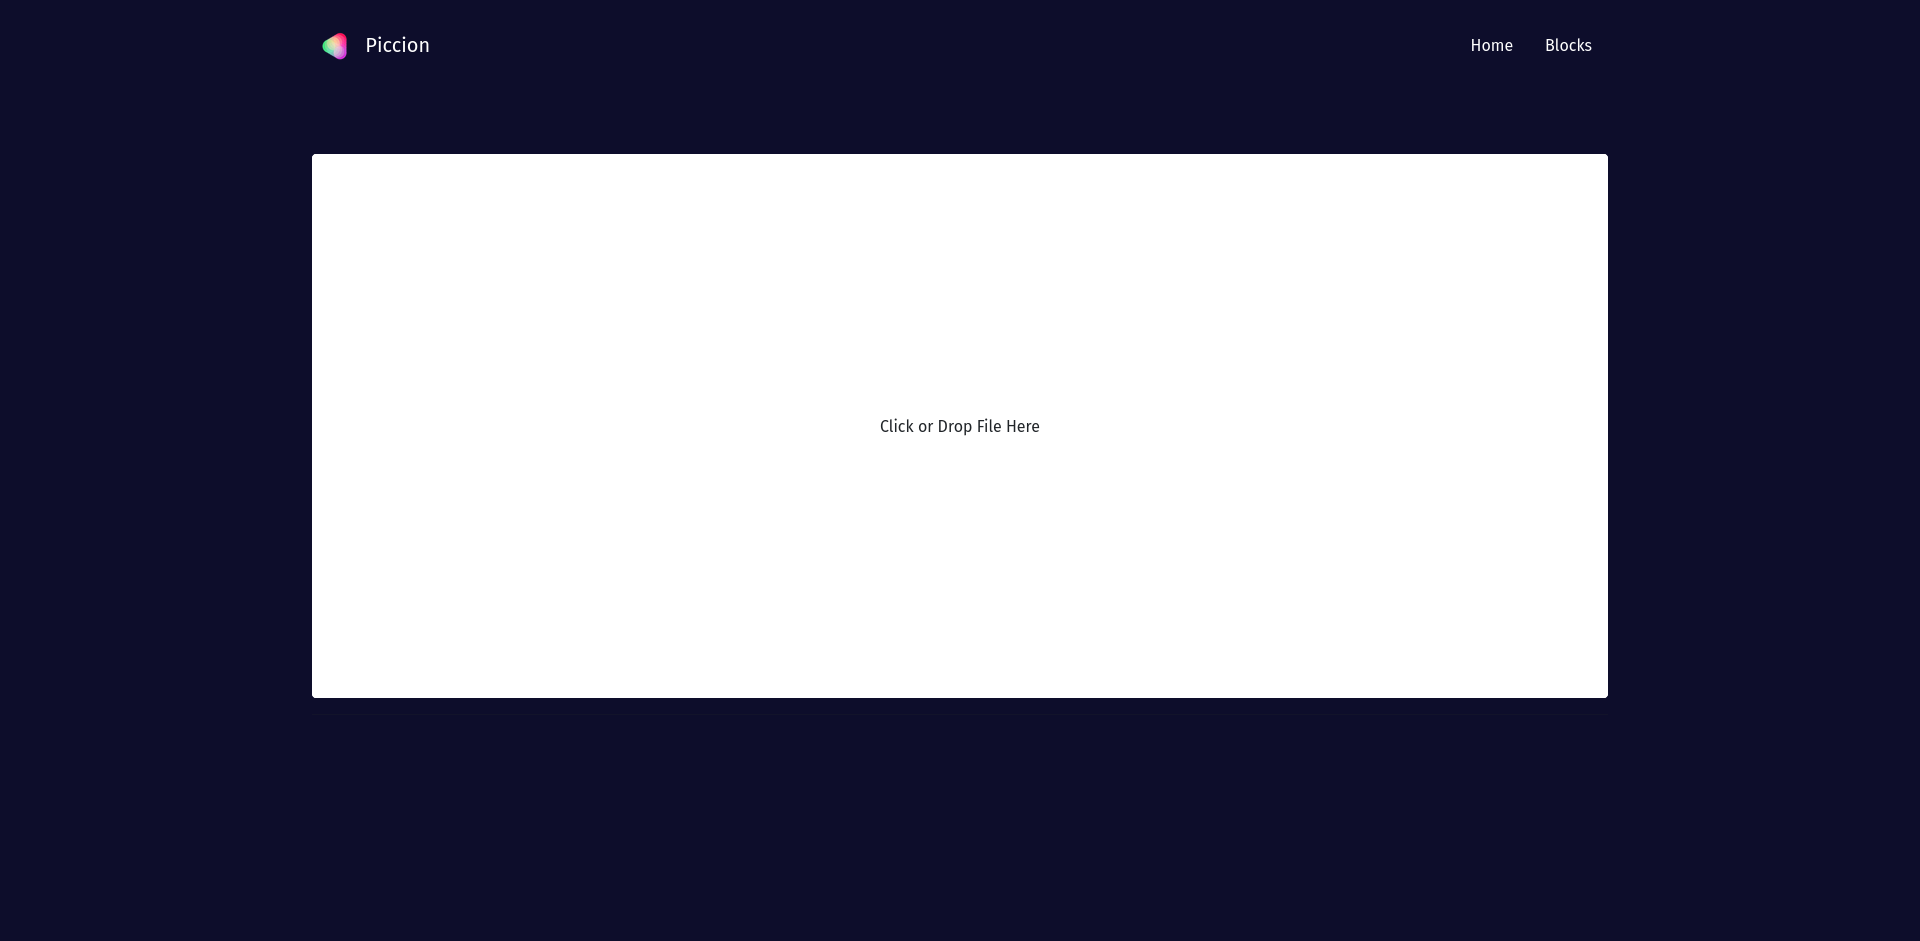
\includegraphics[width=\textwidth]{images/website5.png}

\end{document}